
Of course, to build earable computing systems, we must understand and analyze
characteristics of earable applications.  In this work, through a survey of
research literature and recent practice, and conversations with earable computing domain experts,
%and our own experience with building and prototyping application specific
%systems, 
we will first identify a set of computation tasks that may be common across
a variety of earable applications.  We will then identify, through
a survey of papers discussing implementations of these tasks, a set of
algorithms that often underpin these tasks.  We will then understand through
profiling-based measurements the computational characteristics of these
algorithms.  An understanding of these
characteristics can be used to build and optimize earable computing systems for different
system-level constraints.


\begin{table}[]
\label{tab:earbench}
\caption{Representative earable applications: Inputs, outputs and timing requirements.}
\tiny
\begin{tabular}{ll}
\toprule
Applications    & Inputs / Outputs / Timing Requirements  \\ \midrule
tinySR          & 1s audio /
Small vocabulary English words
/ real time ($\leq \SI{1}{\second}$)   \\
DeepSpeech      & 5s audio /
English text
/ real time ($\leq \SI{1}{\second}$)   \\
Ambisonic-2/6/8     & 10s audio /
Binauralized audio
/ real time ($\leq \SI{1}{\second}$)   \\
HMT-1           & IMU@\SI{100}{\hertz} /
dead-reckoned location of the user
/  $\leq \SI{1}{\second}$             \\
HMT-10          & IMU@\SI{1}{\kilo\hertz} /
dead-reckoned location of the user
/ $\leq \SI{1}{\second}$               \\
HRTF - 2/6/8    &  8sec audio / binauralized audio /   $\leq \SI{1}{\second}$ \\
Speaker Auth.   & 1s audio /
Classifies the speaker as one of the 10 authorized speakers,\\
& or as unauthorized
/ real time ($\leq \SI{1}{\second}$)    \\
ALBERT          & question (10 words) /
start\_logits: the logits of being \\
& the start of the answer of each position
end\_logits: the logits of being \\
& the end of the answer of each position.
/  $\leq \SI{3}{\second}$\\
DeepECGCNN      & 9s ECG signal  /
Four output classes 1) Normal sinus rhythm, 2) Arrhythmic, \\
& 3) Other kind
of rhythm,
4) Very noisy,
/ 9s                    \\
Wave2Letter     &  MFCC with input tensor share (1, 296, 39)
/ Tensor of time and class probability of shape \\
& (1, 1, 148, 29)
/ real time ($\leq \SI{1}{\second}$)  \\
TLIO-1DResNet18 & IMU@200HZ/
Two 3D vectors, the displacement estimates and their \\
& uncertainties
/ $\leq \SI{0.1}{\second}$/inference \\
EKF & IMU data 75k samples / Orientation of IMU /  $\leq \SI{1}{\second}$\\
\bottomrule
\end{tabular}
\label{tab:requirements}
\end{table}

As preliminary analysis,
we conducted a comprehensive survey of earable applications research and
practice~\cite{}, including over 50 papers on http://esense.io, and interviewed
three earable computing domain experts. We observed that most research and
commercial earable computing applications fall into one of four categories: (1)
Human-Machine Interface (HMI) applications that allow the earable user to
interact with the device (and vice-versa). In the absence of traditional
interfaces (e.g., keyboard, mouse, touchscreen), interactions are typically via
sound and taps. (2) Audio applications that decode, manipulate, and playback
audio data streams (e.g., phone calls, podcasts, acoustic augmented reality
(AAR)). (3) Analytics applications, such as ECG monitors, that are
computation-heavy but should ideally execute locally on the earable device.
Finally, (4) Spatial Awareness applications that localize the user, their
movements, head gestures, etc. for applications in AR/VR, gaming, location-
specific alerts, etc. These spatial tracking applications are often
characterized by sensor fusion engines, and are thus assigned to a separate
category. To have a representative, but diverse suite, we then selected from
each category 2-4 applications with different computational requirements, as
determined by profiling (Table~\ref{tab:earbench_metrics}), and diverse
sensor-based inputs. Diversity was considered also in terms of underlying
algorithms (e.g., DSP vs ML, RNN vs CNN vs BERT) and use cases (e.g.,
authentication vs recognition, classification vs NLP, tracking vs
localization).

We will continue the analysis to finalize the list of representative computational tasks and then build EarSuite --- the first earable computing benchmark suite --- by porting
    all benchmark code to C and OpenMP, designing representative inputs for
    each benchmark, and providing baselines on existing systems. 
    %We will enable
    %EarSuite evaluations for heterogeneous systems --- both heterogeneous
    %SoCs, as well as multi-chip and even multi-device systems.  
    EarSuite
    --- software, data, \& build scripts --- as well as executable binaries
    for major platforms --- will be published under an open source license in
    order to enable commercial and academic research in earable computing.
%    EarBench will consist of a diverse and representative set of current and
 %   future earable computing applications.  
 Data inputs will be drawn from
    real world inputs (e.g., measured microphone, accelerometer, \& ECG data),
    popular queries to current question-answering systems (e.g., Alexa,
    Google Assistant, etc.).

    EarSuite will be published with a CMake based build system.  As CMake
    is an open-source, cross platform build automation tool targeting all
    major operating systems, and since nearly all computer architectures
    have open source or proprietary C compilers, researchers will be able
    to get EarSuite running on a wide variety of systems quickly and easily.
    For major architectures (e.g., ARMv7, ARMv8, x86\_64, i686, etc.),
    we will provide prebuilt EarSuite binaries.

The next goal is to explore computer architectures for earable processing. Naturally, the question arises --
%Are today's hardware platforms not good enough to support earable applications? Second, 
what are the key computational characteristics that any earable computing platform should target?
% We analyze the EarBench suite to identify the key
% computation kernels in earable  applications.
 Figure~\ref{fig:kernels_breakdown} shows the performance breakdown of some representative applications
 across constituent kernels on a single Cortex A72 (profiling was performed on Raspberry Pi 4).  Applications were
 compiled with gcc 9.2 and rustc 1.5 with `O3' optimizations (which include
 SIMD auto-vectorization).
 
 
 
\begin{figure}[h]
  \centering
%   \includegraphics[height=\linewidth,
%   width=1.1\linewidth]{images/kernelsbreakdown.png}
  
    \scalebox{0.65}{% This file was created by tikzplotlib v0.9.8.
\begin{tikzpicture}

\definecolor{color0}{rgb}{0.298039215686275,0.447058823529412,0.690196078431373}
\definecolor{color1}{rgb}{0.866666666666667,0.517647058823529,0.32156862745098}
\definecolor{color2}{rgb}{0.333333333333333,0.658823529411765,0.407843137254902}
\definecolor{color3}{rgb}{0.768627450980392,0.305882352941176,0.32156862745098}
\definecolor{color4}{rgb}{0.505882352941176,0.447058823529412,0.701960784313725}
\definecolor{color5}{rgb}{0.576470588235294,0.470588235294118,0.376470588235294}
\definecolor{color6}{rgb}{0.854901960784314,0.545098039215686,0.764705882352941}

\begin{axis}[
axis background/.style={fill=white!94.1176470588235!black},
axis line style={white!94.1176470588235!black},
legend cell align={left},
legend style={
  fill opacity=0.8,
  draw opacity=1,
  text opacity=1,
  at={(1,0.8)},
  anchor=north west,
  draw=white!80!black,
  fill=white!94.1176470588235!black
},
tick align=outside,
tick pos=left,
x grid style={white!79.6078431372549!black},
xmin=-0.775, xmax=10.775,
xtick style={color=black},
xtick={0,1,2,3,4,5,6,7,8,9,10},
xticklabel style={rotate=90.0},
xticklabels={
\apptinysr{},
\appdeepspeech{},
\appambisonic{},
\apphmt{},
\apphrtf{},
\appspeakerauthentication{},
\appalbert{},
\appdeepecgcnn{},
\appwavetoletter{},
\appresnet{},
\appekf{}
},
y grid style={white!79.6078431372549!black},
ymajorgrids,
ymin=0, ymax=105,
ytick style={color=black}
]
\draw[draw=white,fill=color0,very thin] (axis cs:-0.25,0) rectangle (axis cs:0.25,40.83);
\addlegendimage{only marks,mark=square*,mark options={mark size=4pt,solid, line width=0.5pt},draw=white,fill=color0,very thin};
\addlegendentry{\kernelfft{}}

\draw[draw=white,fill=color1,very thin] (axis cs:-0.25,40.83) rectangle (axis cs:0.25,75.19);
\addlegendimage{only marks,mark=square*,mark options={mark size=4pt,solid, line width=0.5pt},draw=white,fill=color1,very thin};
\addlegendentry{\kernelconvd{}}

\draw[draw=white,fill=color2,very thin] (axis cs:-0.25,75.19) rectangle (axis cs:0.25,75.19);
\addlegendimage{only marks,mark=square*,mark options={mark size=4pt,solid, line width=0.5pt},draw=white,fill=color2,very thin};
\addlegendentry{\kernelgemm{}}

\draw[draw=white,fill=color3,very thin] (axis cs:-0.25,75.19) rectangle (axis cs:0.25,75.19);
\addlegendimage{only marks,mark=square*,mark options={mark size=4pt,solid, line width=0.5pt},draw=white,fill=color3,very thin};
\addlegendentry{\kernelgemv{}}

\draw[draw=white,fill=color4,very thin] (axis cs:-0.25,75.19) rectangle (axis cs:0.25,75.19);
\addlegendimage{only marks,mark=square*,mark options={mark size=4pt,solid, line width=0.5pt},draw=white,fill=color4,very thin};
\addlegendentry{\kernelbilinear{}}

\draw[draw=white,fill=color5,very thin] (axis cs:-0.25,75.19) rectangle (axis cs:0.25,75.19);
\addlegendimage{only marks,mark=square*,mark options={mark size=4pt,solid, line width=0.5pt},draw=white,fill=color5,very thin};
\addlegendentry{\kernelconvdd{}}

\draw[draw=white,fill=color6,very thin] (axis cs:-0.25,75.19) rectangle (axis cs:0.25,75.19);
\addlegendimage{only marks,mark=square*,mark options={mark size=4pt,solid, line width=0.5pt},draw=white,fill=color6,very thin};
\addlegendentry{\kernellu{}}

\draw[draw=white,fill=white!54.9019607843137!black,very thin] (axis cs:-0.25,75.19) rectangle (axis cs:0.25,100);
\addlegendimage{only marks,mark=square*,mark options={mark size=4pt,solid, line width=0.5pt},draw=white,fill=white!54.9019607843137!black,very thin};
\addlegendentry{\kernelrest{}}

\draw[draw=white,fill=color0,very thin] (axis cs:0.75,0) rectangle (axis cs:1.25,0);
\draw[draw=white,fill=color1,very thin] (axis cs:0.75,0) rectangle (axis cs:1.25,0);
\draw[draw=white,fill=color2,very thin] (axis cs:0.75,0) rectangle (axis cs:1.25,86.37);
\draw[draw=white,fill=color3,very thin] (axis cs:0.75,86.37) rectangle (axis cs:1.25,86.37);
\draw[draw=white,fill=color4,very thin] (axis cs:0.75,86.37) rectangle (axis cs:1.25,86.37);
\draw[draw=white,fill=color5,very thin] (axis cs:0.75,86.37) rectangle (axis cs:1.25,86.37);
\draw[draw=white,fill=color6,very thin] (axis cs:0.75,86.37) rectangle (axis cs:1.25,86.37);
\draw[draw=white,fill=white!54.9019607843137!black,very thin] (axis cs:0.75,86.37) rectangle (axis cs:1.25,100);
\draw[draw=white,fill=color0,very thin] (axis cs:1.75,0) rectangle (axis cs:2.25,71.99);
\draw[draw=white,fill=color1,very thin] (axis cs:1.75,71.99) rectangle (axis cs:2.25,71.99);
\draw[draw=white,fill=color2,very thin] (axis cs:1.75,71.99) rectangle (axis cs:2.25,71.99);
\draw[draw=white,fill=color3,very thin] (axis cs:1.75,71.99) rectangle (axis cs:2.25,71.99);
\draw[draw=white,fill=color4,very thin] (axis cs:1.75,71.99) rectangle (axis cs:2.25,71.99);
\draw[draw=white,fill=color5,very thin] (axis cs:1.75,71.99) rectangle (axis cs:2.25,71.99);
\draw[draw=white,fill=color6,very thin] (axis cs:1.75,71.99) rectangle (axis cs:2.25,71.99);
\draw[draw=white,fill=white!54.9019607843137!black,very thin] (axis cs:1.75,71.99) rectangle (axis cs:2.25,100);
\draw[draw=white,fill=color0,very thin] (axis cs:2.75,0) rectangle (axis cs:3.25,0);
\draw[draw=white,fill=color1,very thin] (axis cs:2.75,0) rectangle (axis cs:3.25,0);
\draw[draw=white,fill=color2,very thin] (axis cs:2.75,0) rectangle (axis cs:3.25,15.47);
\draw[draw=white,fill=color3,very thin] (axis cs:2.75,15.47) rectangle (axis cs:3.25,30.8);
\draw[draw=white,fill=color4,very thin] (axis cs:2.75,30.8) rectangle (axis cs:3.25,30.8);
\draw[draw=white,fill=color5,very thin] (axis cs:2.75,30.8) rectangle (axis cs:3.25,30.8);
\draw[draw=white,fill=color6,very thin] (axis cs:2.75,30.8) rectangle (axis cs:3.25,30.8);
\draw[draw=white,fill=white!54.9019607843137!black,very thin] (axis cs:2.75,30.8) rectangle (axis cs:3.25,100);
\draw[draw=white,fill=color0,very thin] (axis cs:3.75,0) rectangle (axis cs:4.25,80.11);
\draw[draw=white,fill=color1,very thin] (axis cs:3.75,80.11) rectangle (axis cs:4.25,80.11);
\draw[draw=white,fill=color2,very thin] (axis cs:3.75,80.11) rectangle (axis cs:4.25,80.11);
\draw[draw=white,fill=color3,very thin] (axis cs:3.75,80.11) rectangle (axis cs:4.25,80.11);
\draw[draw=white,fill=color4,very thin] (axis cs:3.75,80.11) rectangle (axis cs:4.25,87.76);
\draw[draw=white,fill=color5,very thin] (axis cs:3.75,87.76) rectangle (axis cs:4.25,87.76);
\draw[draw=white,fill=color6,very thin] (axis cs:3.75,87.76) rectangle (axis cs:4.25,87.76);
\draw[draw=white,fill=white!54.9019607843137!black,very thin] (axis cs:3.75,87.76) rectangle (axis cs:4.25,100);
\draw[draw=white,fill=color0,very thin] (axis cs:4.75,0) rectangle (axis cs:5.25,21.597);
\draw[draw=white,fill=color1,very thin] (axis cs:4.75,21.597) rectangle (axis cs:5.25,48.648);
\draw[draw=white,fill=color2,very thin] (axis cs:4.75,48.648) rectangle (axis cs:5.25,54.581);
\draw[draw=white,fill=color3,very thin] (axis cs:4.75,54.581) rectangle (axis cs:5.25,54.581);
\draw[draw=white,fill=color4,very thin] (axis cs:4.75,54.581) rectangle (axis cs:5.25,54.581);
\draw[draw=white,fill=color5,very thin] (axis cs:4.75,54.581) rectangle (axis cs:5.25,54.581);
\draw[draw=white,fill=color6,very thin] (axis cs:4.75,54.581) rectangle (axis cs:5.25,54.581);
\draw[draw=white,fill=white!54.9019607843137!black,very thin] (axis cs:4.75,54.581) rectangle (axis cs:5.25,100);
\draw[draw=white,fill=color0,very thin] (axis cs:5.75,0) rectangle (axis cs:6.25,0);
\draw[draw=white,fill=color1,very thin] (axis cs:5.75,0) rectangle (axis cs:6.25,0);
\draw[draw=white,fill=color2,very thin] (axis cs:5.75,0) rectangle (axis cs:6.25,0);
\draw[draw=white,fill=color3,very thin] (axis cs:5.75,0) rectangle (axis cs:6.25,87.49);
\draw[draw=white,fill=color4,very thin] (axis cs:5.75,87.49) rectangle (axis cs:6.25,87.49);
\draw[draw=white,fill=color5,very thin] (axis cs:5.75,87.49) rectangle (axis cs:6.25,87.49);
\draw[draw=white,fill=color6,very thin] (axis cs:5.75,87.49) rectangle (axis cs:6.25,87.49);
\draw[draw=white,fill=white!54.9019607843137!black,very thin] (axis cs:5.75,87.49) rectangle (axis cs:6.25,100);
\draw[draw=white,fill=color0,very thin] (axis cs:6.75,0) rectangle (axis cs:7.25,0);
\draw[draw=white,fill=color1,very thin] (axis cs:6.75,0) rectangle (axis cs:7.25,0);
\draw[draw=white,fill=color2,very thin] (axis cs:6.75,0) rectangle (axis cs:7.25,0);
\draw[draw=white,fill=color3,very thin] (axis cs:6.75,0) rectangle (axis cs:7.25,2.65);
\draw[draw=white,fill=color4,very thin] (axis cs:6.75,2.65) rectangle (axis cs:7.25,2.65);
\draw[draw=white,fill=color5,very thin] (axis cs:6.75,2.65) rectangle (axis cs:7.25,94.48);
\draw[draw=white,fill=color6,very thin] (axis cs:6.75,94.48) rectangle (axis cs:7.25,94.48);
\draw[draw=white,fill=white!54.9019607843137!black,very thin] (axis cs:6.75,94.48) rectangle (axis cs:7.25,100);
\draw[draw=white,fill=color0,very thin] (axis cs:7.75,0) rectangle (axis cs:8.25,0);
\draw[draw=white,fill=color1,very thin] (axis cs:7.75,0) rectangle (axis cs:8.25,0);
\draw[draw=white,fill=color2,very thin] (axis cs:7.75,0) rectangle (axis cs:8.25,0);
\draw[draw=white,fill=color3,very thin] (axis cs:7.75,0) rectangle (axis cs:8.25,0);
\draw[draw=white,fill=color4,very thin] (axis cs:7.75,0) rectangle (axis cs:8.25,0);
\draw[draw=white,fill=color5,very thin] (axis cs:7.75,0) rectangle (axis cs:8.25,97.76);
\draw[draw=white,fill=color6,very thin] (axis cs:7.75,97.76) rectangle (axis cs:8.25,97.76);
\draw[draw=white,fill=white!54.9019607843137!black,very thin] (axis cs:7.75,97.76) rectangle (axis cs:8.25,100);
\draw[draw=white,fill=color0,very thin] (axis cs:8.75,0) rectangle (axis cs:9.25,0);
\draw[draw=white,fill=color1,very thin] (axis cs:8.75,0) rectangle (axis cs:9.25,0);
\draw[draw=white,fill=color2,very thin] (axis cs:8.75,0) rectangle (axis cs:9.25,85.71);
\draw[draw=white,fill=color3,very thin] (axis cs:8.75,85.71) rectangle (axis cs:9.25,85.71);
\draw[draw=white,fill=color4,very thin] (axis cs:8.75,85.71) rectangle (axis cs:9.25,85.71);
\draw[draw=white,fill=color5,very thin] (axis cs:8.75,85.71) rectangle (axis cs:9.25,85.71);
\draw[draw=white,fill=color6,very thin] (axis cs:8.75,85.71) rectangle (axis cs:9.25,85.71);
\draw[draw=white,fill=white!54.9019607843137!black,very thin] (axis cs:8.75,85.71) rectangle (axis cs:9.25,100);
\draw[draw=white,fill=color0,very thin] (axis cs:9.75,0) rectangle (axis cs:10.25,0);
\draw[draw=white,fill=color1,very thin] (axis cs:9.75,0) rectangle (axis cs:10.25,0);
\draw[draw=white,fill=color2,very thin] (axis cs:9.75,0) rectangle (axis cs:10.25,23.14);
\draw[draw=white,fill=color3,very thin] (axis cs:9.75,23.14) rectangle (axis cs:10.25,39.36);
\draw[draw=white,fill=color4,very thin] (axis cs:9.75,39.36) rectangle (axis cs:10.25,39.36);
\draw[draw=white,fill=color5,very thin] (axis cs:9.75,39.36) rectangle (axis cs:10.25,39.36);
\draw[draw=white,fill=color6,very thin] (axis cs:9.75,39.36) rectangle (axis cs:10.25,42.47);
\draw[draw=white,fill=white!54.9019607843137!black,very thin] (axis cs:9.75,42.47) rectangle (axis cs:10.25,100);
\end{axis}

\end{tikzpicture}

}
  \caption{\small Constituent kernels of representative earable applications.}
%  \vspace{-7mm}
    \label{fig:kernels_breakdown}
\end{figure}


Figure~\ref{fig:kernels_breakdown} shows that earable applications are
built out of a small number of computationally intensive DSP and ML
kernels.  At first glance, this commonality of kernels in applications
%crossing four taxonomic categories, with
across  a wide range of use-cases (e.g., audio playback, text processing,
heart-rate monitoring, speech processing, etc.) may seem surprising.
However, note that these applications are implemented broadly using techniques from digital signal processing and machine learning; 
%DSP and ML computation are well-known to both be dominated by a small number of computation kernels and share  computation kernels between them~\cite{narayan2019novel}. 
%\nathan{
Machine learning and DSP kernels have similar computation.
A neural network consists of an alternating sequence of linear transformations and non-linear activation functions. Computing the action of a linear transformation, $W$, on an input vector, $a$, is given by $b = Wa$.  Given a choice of basis, $W$ and $a$ can be expressed in matrix form, and computing the $i$'th output of $b$ is
\begin{equation}
    b_i = \sum_{n=0}^{N-1} a_jW_{ij}.
\end{equation}
Similarly, computing the $N$-point discrete Fourier transform (DFT) of a real or complex vector, $x$, is given by the linear transformation $X = Wx$, and $W_{nk} = e^{-i2\pi/N}$ is an element of the order $N$ subgroup of the unit circle group.
Thus, the `frequency-domain' output
\begin{equation}
   X[k] = \sum_{n=0}^{N-1} x[n] W_{nk}
\end{equation}
is remarkably similar to the core computation of a neural network.
Two factors complicate using a substrate optimized for ML kernels to be used for DSP kernels and vice versa. First, neural networks typically are real-valued, while DFT is complex valued.  Second, symmetries in the DFT's transformation enable a `fast' $O(n\log n)$ Fourier transform by recursively subdividing the $N$-point DFT into smaller and smaller sub-blocks.  Similarly, neural networks often exploit symmetries of their own to greatly reduce required computation and data movement by using convolution layers.
Despite these complications, striking similarities remain.  Both DFT and neural network computations are made up of real-valued multiplications followed by additions/subtractions, and in both the number of multiplications needed is nearly identical to the number of additions/subtractions needed. This suggests that an efficient processor architecture for earable applications is a neural network accelerator that is augmented with support for complex processing and that can be reconfigured to support different dataflows for the different ML and DSP kernels. 

Furthermore, since the dataflows of dot-product and complex multiplication, the key subcomputations of neural networks and FFT, respectively, consist of scattering
data streams to multiplication units, followed by reduction (dot-product) and gathering into an output stream (complex multiplication), an architecture which enables scatter-multiply-reduce and scatter-multiply-gather is needed
(Figure~\ref{fig:complex-vs-dot}).
High bandwidth tree-structures for both the scatter network, and for the reduction/gather network should enable efficient computation of machine learning and DSP workloads.

\begin{figure}[htbp]
 \centering
   \subfloat{
   {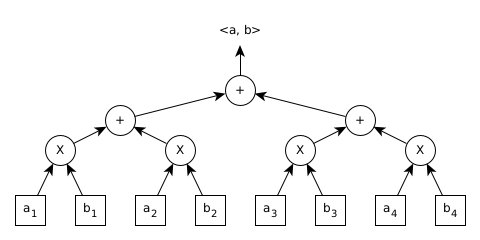
\includegraphics[width=0.48\linewidth]{dot_prod_dataflow.png}}
   }
   \subfloat{
   {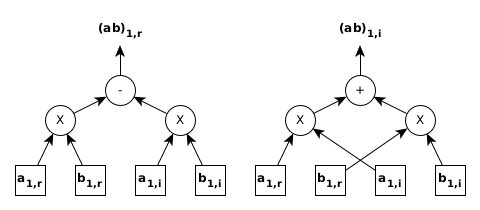
\includegraphics[width=0.48\linewidth]{complex_multiply_dataflow.png}}
   }
   %\label{fig:complex-vs-dot}
   \caption{
   \small
   Dataflows for dot-product (left) and complex multiplication (right).
 }
% \vspace{-5mm}
 \label{fig:complex-vs-dot}
 %\label{fig:vm-configs}
\end{figure}




Many classes of programmable hardware, such as GPUs and DSPs, already
accelerate a variety of DSP and ML kernels. However, they draw high power
(e.g., \SI{234}{\milli\watt} for HiFi4 DSP, 1.8W for Mali T628 MP6 GPU vs tens
of \si{\milli\watt}s required for earable hardware) due to their excessive
generality. 
For example, GPUs use expensive floating point
arithmetic (vs fixed point arithmetic that may be adequate for earable
computing kernels), general-purpose microarchitecture (earable applications may largely need only a tree of adders and multipliers customized to the earable ML/DSP kernels), and
dedicated graphics pipelines (that unnecessarily contribute static power in
context of earable computing). 

ML accelerators are not a good fit either
since it is unclear how to map earable DSP kernels such as LU, Bilinear, Cholesky, and FFT on such hardware (due to lack of
support for non-matrix computation, vectorized complex operations, or non-multiply or add
operations, for example). 

\begin{figure}[h]
  \centering
  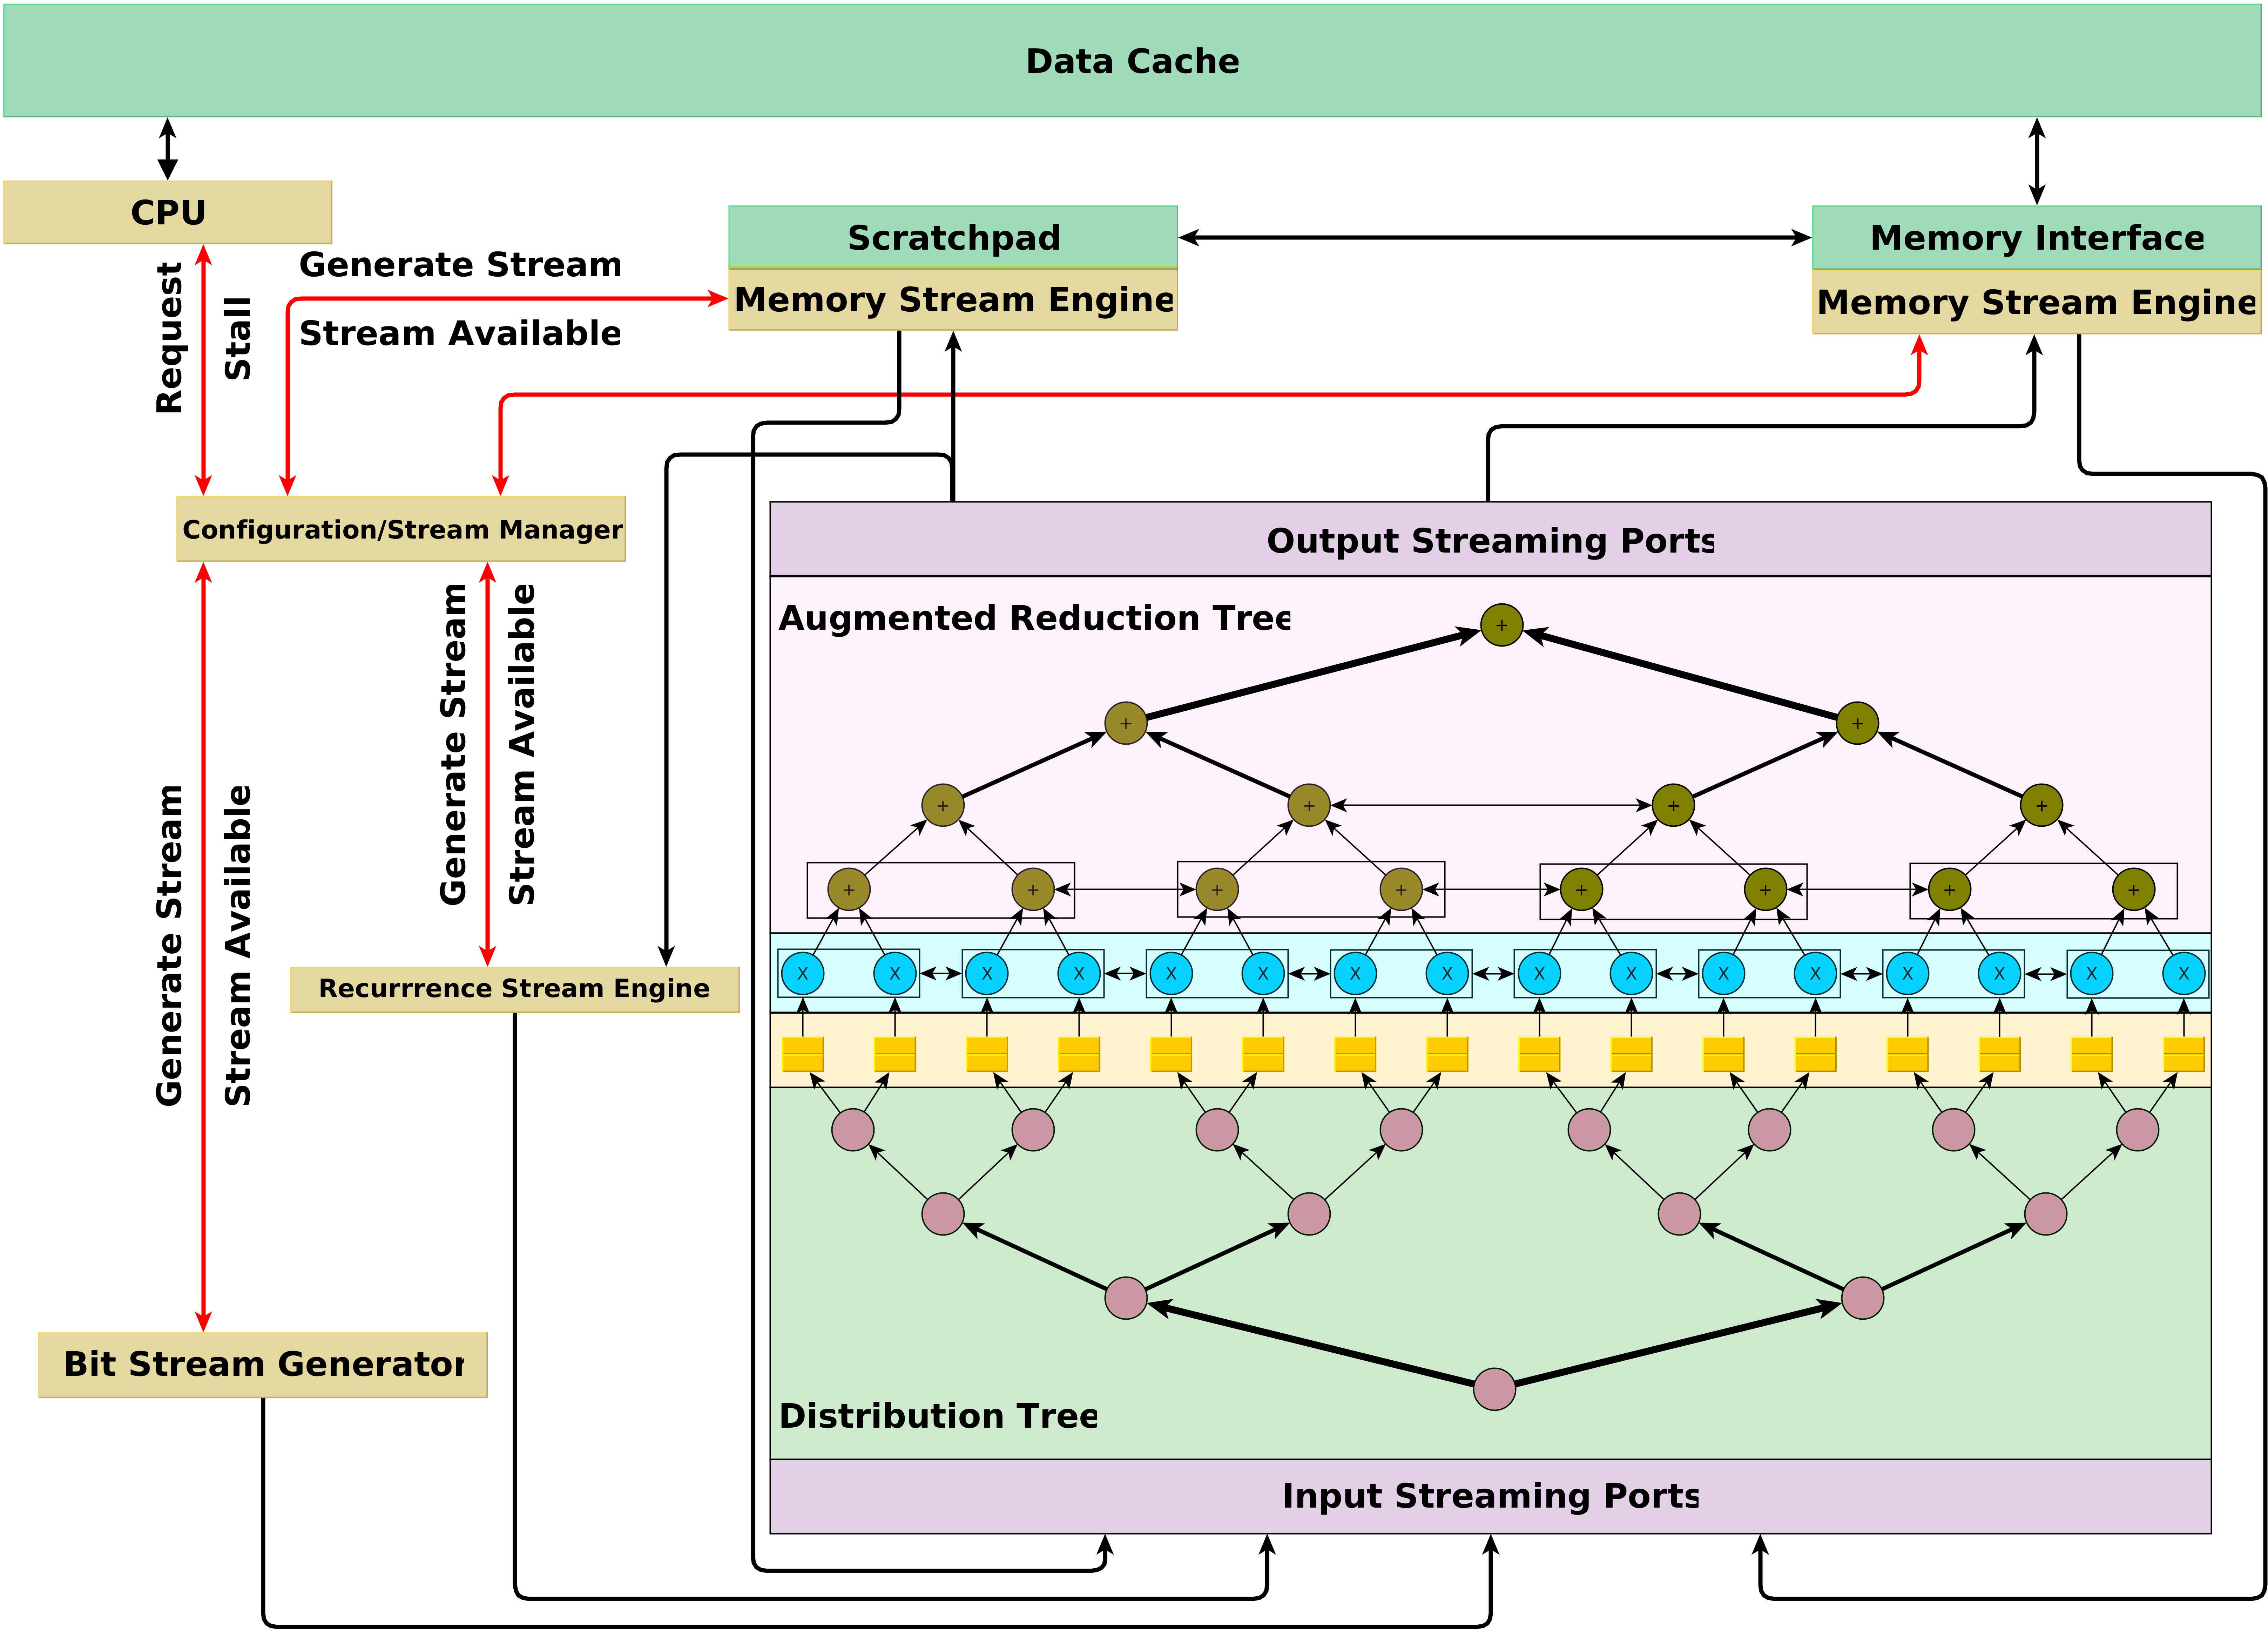
\includegraphics[width=0.48\textwidth]{arch.png}
  %\includesvg[height=\linewidth,width=\textwidth]{images/arch.svg}
  \caption{
  \small
  Architecture of \arch{}.}
  \label{fig:arch}
\end{figure}

 We will use EarSuite to drive a design space exploration of computer architectures for earable processing. An example computer architecture (that we have preliminarily explored~\cite{}) is  a
stream-programmed~\cite{nowatzki2017stream} coarse-grained reconfigurable
spatial architecture (Figure~\ref{fig:earable_arch}) whose 
computation substrate consists of a set of  adders and multipliers (since earable applications are dominated by inner-product-based computation).
 A fat distribution
tree~\cite{leiserson1985fat}  feeds the multiplier units.  The products
of the multiplier units are forwarded to the adders organized in an `augmented
reduction tree', which allows a single tree to perform multiple inner
products concurrently, or to be time-multiplexed to perform a large inner-product across multiple cycles.
The final few adder units are equipped
with accumulators to enable computation of multiple inner-products in parallel. The accumulators may be configured to output either
the accumulated value, $x$, or $\max{\{0, x\}}$, such that the architecture supports
either linear or reLU activation functions.  Max-pooling
layers is supported through the reduction tree by allowing the adder units to also perform
comparison operations.
 The architecture  uses  32-bit fixed-point arithmetic since high quality audio
often has a 24-bit depth, while 16-bit fixed-point arithmetic would %necessarily
lower audio quality. 
Furthermore, since FFT is a key computational kernel in earable application, the
functional units support vectorized complex operations. To enable 
multiplication of complex numbers, two adjacent multipliers form a pair to create a  {\em
logical vector multiplier}.
%which perform complex multiplication and
%addition on streams of complex numbers (in array-of-structs form). In order to
%support this the vectorized PEs 
Each logical vector multiplier can be configured to either perform a 2x32 bit multiplication or a 2x32 bit
multiplication in which one of the 64-bit inputs' top and bottom 32-bits are
swapped.
Also, since $i^2 = -1$, the real component of
the complex product is produced by computing the difference
of two of the partial products while the imaginary component is produced by
computing the sum of the other two partial products. To support this,  adjacent adders in level 3 of the tree
form  \textit{logical vector adders}. The `left' adder in a logical vector adder can
be configured to perform subtraction as well as addition.
The control core executes code that does not fit
well on the reconfigurable substrate, including non-multiply
or add operations in the DSP kernel code (e.g., square-root and divide operations in LU and Cholesky). 

There are several other computer architectures possible as well. 
One possibility is to support multiple fixed function accelerators on the earable SoC each targeting a different set of kernels. For example, an SoC with a CPU, an ML accelerator, and an FFT accelerator looks attractive for our applications. However, there are several disadvantages of such an approach. One, the field of earable computing is relatively new and algorithms are still evolving. Any system with fixed functions ASICs may become obsolete quickly. 
Second,  
a collection of special purpose accelerators will fail to provide the requisite performance for kernels that do not map well to an existing accelerator. For example, LU, Bilinear, and Cholesky cannot be mapped directly on an ML accelerator or an FFT accelerator and will need to be run on the CPU at high performance cost. Similarly, a given kernel may not fit its fixed function accelerator well depending on the input. For example, FFT size in tinySR, depends on input audio length and, for our
microphone input, varies from 32-point to 
1024-point, HRTF calls a 4096-point FFT, Ambisonic uses a 512 or 1024-point FFT, etc. Many FFT accelerators are optimized for a specific size~\cite{fft01} and will not run other FFTs of other sizes efficiently~\cite{fft02}. 
Nevertheless, a heterogeneous system has benefits in terms of reusability and cost. We will compare the spatial approaches against heterogeneous approaches.

We will also prototype and test an earable computer in TSMC \(\leq
    \SI{65}{\nano\meter}\) technology.
    The candidate design, the spatial architecture described above, shows
    significant performance and energy improvement over existing hardware
    systems used in today's earable computers.
    Prototyping sub-objectives include physical design of the architecture to minimize energy, including
        design and placement of multiple power and clock domains, integration
        of the architecture with commercially licensable SRAMs to minimize cost, and design
        for test, chip tape-out, and packaging for workforce development.  Multiple power domains are
        used as the architecture is a heterogeneous system (control core and reconfigurable substrate), and thus power gating can be
        used to reduce static power consumption. Similarly, clock and voltage
        scaling can be used minimize energy or power consumption when one or
        more of the architecture's components has performance slack available.  
        Although we have a preliminary architecture,
        %SpEaC's architecture and preliminary design are complete, architectural
        %research 
        a careful exploration would be needed to determine the optimal choice of operating points.   Similarly, testing sub-objectives include earable system design
        and PCB design, porting EarSuite applications to the chip, and collecting
        measured EarSuite results.  System design will incorporate multiple
        earable sensors (e.g., microphone arrays, inertial motion units),
        actuators (e.g., speakers, antennae), and a hardware debug system.
        Porting EarSuite applications to the chip requires annotating the EarSuite
        C code with pragmas which enable the architecture's compiler to automatically
        generate configurations and data streams for its spatial accelerator.
        PI Kumar is experienced in digital design, chip design,
        tape-out and testing, and runs an undergraduate course in which
        students design and tape-out processors which are manufactured by TSMC
        and then tested at UIUC campus.  His research group also participates
        in Intel's Chip Design Challenge, in manufacturing RISC-V processors in
        Intel's \SI{16}{\nano\meter} technology. The research group has also recently taped out several flexible chips~\cite{}.


\begin{figure}[htbp]
  \centering
    \subfloat{
        {\includesvg[width=0.48\linewidth]{kernels.svg}}
        }
    \subfloat{
        {\includesvg[width=0.48\linewidth]{applications.svg}}
    }
    \caption{ Communication energy of BLE transceiver when inputs and outputs
    are transmitted over BLE for remote compute offloading, normalized with
    respect to the energy consumed when kernels and applications are
    computed locally.}
  \label{fig:ble}
\end{figure}

A natural question comes up: whether to offload compute to 
mobile device (using BLE, for example) - this will involve sending inputs and outputs over the communication protocol - or compute locally on an earable processor? 
 Communication can be expensive. \cite{ble} claims that it takes $8usec$ to communicate one byte of data over BLE whereas the TX power of BLE is 84mW and RX power is 66mW. 
 %We used power and communication latency numbers from \cite{ble} along with the input and output sizes of our kernels and applications and computed the
%energy consumed by the BLE transceiver.
Figure~\ref{fig:ble}-a shows the 
communication energy of BLE transceiver normalized with respect to the energy consumed by the above proposed spatial architecture when we run the kernels locally on the architecture. Our results show that 
computing kernels locally is on average $\approx4OOM$ more energy efficient compared to communicating inputs/outputs over BLE. This is not surprising since BLE
%although BLE is low power protocol, it 
consumes significant amount of energy ($\approx\SI{0.7}{\micro\joule\per\byte}$~\cite{ble}) when sending large matrices, which are common inputs to our kernels, due to its long communication latency.
Similarly, figure~\ref{fig:ble}-b shows the 
communication energy of BLE transceiver normalized with respect to the energy consumed by the spatial architecture when we run the entire application locally. The results show that 
for compute intensive applications, e.g. Albert, it is more energy efficient to offload compute to remote device,
whereas for all other applications 
computing applications locally is more energy efficient than offloading the compute to remote device over BLE.
On average computing locally  is $\approx12.7\times$ more energy efficient across applications we considered compared to communicating inputs/outputs over BLE. 
%Another possibility is to offload computation to a remote, non-earable device. However, this leads to concerns about energy (since energy of transmitting
%    data wirelessly via BLE is orders of magnitude greater than transmitting
%    data to/from local memory, 
Other than energy benefits, local computation may often be preferred also for improved 
%as well as 
latency, privacy, and usability (since a remote device may not always be available or accessible).

At the same time, applications such as Albert which have high computation and memory requirements may need to be offloaded to a remote device both for energy and capability reasons. We will analyze both proposed hardware and existing earable hardware in a heterogeneous, networked computational settings, in which computation can be offloaded from the earable device onto a number of other devices, including smart watches,  smart phones, and high performance cloud systems. We will use HPVM~\cite{} for distributed implementation of the EarSuite benchmarks. The distributed implementations will be open sourced and released publicly. 
%\end{enumerate}
